\documentclass{article}\usepackage{graphicx, color}
%% maxwidth is the original width if it is less than linewidth
%% otherwise use linewidth (to make sure the graphics do not exceed the margin)
\makeatletter
\def\maxwidth{ %
  \ifdim\Gin@nat@width>\linewidth
    \linewidth
  \else
    \Gin@nat@width
  \fi
}
\makeatother

\IfFileExists{upquote.sty}{\usepackage{upquote}}{}
\definecolor{fgcolor}{rgb}{0.2, 0.2, 0.2}
\newcommand{\hlnumber}[1]{\textcolor[rgb]{0,0,0}{#1}}%
\newcommand{\hlfunctioncall}[1]{\textcolor[rgb]{0.501960784313725,0,0.329411764705882}{\textbf{#1}}}%
\newcommand{\hlstring}[1]{\textcolor[rgb]{0.6,0.6,1}{#1}}%
\newcommand{\hlkeyword}[1]{\textcolor[rgb]{0,0,0}{\textbf{#1}}}%
\newcommand{\hlargument}[1]{\textcolor[rgb]{0.690196078431373,0.250980392156863,0.0196078431372549}{#1}}%
\newcommand{\hlcomment}[1]{\textcolor[rgb]{0.180392156862745,0.6,0.341176470588235}{#1}}%
\newcommand{\hlroxygencomment}[1]{\textcolor[rgb]{0.43921568627451,0.47843137254902,0.701960784313725}{#1}}%
\newcommand{\hlformalargs}[1]{\textcolor[rgb]{0.690196078431373,0.250980392156863,0.0196078431372549}{#1}}%
\newcommand{\hleqformalargs}[1]{\textcolor[rgb]{0.690196078431373,0.250980392156863,0.0196078431372549}{#1}}%
\newcommand{\hlassignement}[1]{\textcolor[rgb]{0,0,0}{\textbf{#1}}}%
\newcommand{\hlpackage}[1]{\textcolor[rgb]{0.588235294117647,0.709803921568627,0.145098039215686}{#1}}%
\newcommand{\hlslot}[1]{\textit{#1}}%
\newcommand{\hlsymbol}[1]{\textcolor[rgb]{0,0,0}{#1}}%
\newcommand{\hlprompt}[1]{\textcolor[rgb]{0.2,0.2,0.2}{#1}}%

\usepackage{framed}
\makeatletter
\newenvironment{kframe}{%
 \def\at@end@of@kframe{}%
 \ifinner\ifhmode%
  \def\at@end@of@kframe{\end{minipage}}%
  \begin{minipage}{\columnwidth}%
 \fi\fi%
 \def\FrameCommand##1{\hskip\@totalleftmargin \hskip-\fboxsep
 \colorbox{shadecolor}{##1}\hskip-\fboxsep
     % There is no \\@totalrightmargin, so:
     \hskip-\linewidth \hskip-\@totalleftmargin \hskip\columnwidth}%
 \MakeFramed {\advance\hsize-\width
   \@totalleftmargin\z@ \linewidth\hsize
   \@setminipage}}%
 {\par\unskip\endMakeFramed%
 \at@end@of@kframe}
\makeatother

\definecolor{shadecolor}{rgb}{.97, .97, .97}
\definecolor{messagecolor}{rgb}{0, 0, 0}
\definecolor{warningcolor}{rgb}{1, 0, 1}
\definecolor{errorcolor}{rgb}{1, 0, 0}
\newenvironment{knitrout}{}{} % an empty environment to be redefined in TeX

\usepackage{alltt}
\usepackage[sc]{mathpazo}
\usepackage{geometry}
\usepackage{graphicx}
\geometry{verbose,tmargin=2.5cm,bmargin=2.5cm,lmargin=2.5cm,rmargin=2.5cm}
\setcounter{secnumdepth}{2}
\setcounter{tocdepth}{2}
\usepackage{url}
\usepackage[unicode=true,pdfusetitle,
 bookmarks=true,bookmarksnumbered=true,bookmarksopen=true,bookmarksopenlevel=2,
 breaklinks=false,pdfborder={0 0 1},backref=false,colorlinks=false]
 {hyperref}
\hypersetup{
 pdfstartview={XYZ null null 1}}
\usepackage{breakurl}
\begin{document}





\title{Tradeoff analysis issues}


\author{Karthik Ram}

\maketitle

A quick summary of the issues with my analysis thus far. Of the three trade offs we chose to evaluate, I am able to run trade off 1 and 3 (briefly described below) but cannot generate any trade off between adult survival and fecundity (trade off #2). I'm fine with leaving it out and just focusing on cleaning up the results from 1 and 3. Here are my last remaining issues. \\

Trade-off 1 (juvenile growth vs survival):  For the simulations on a tradeoff between juvenile growth and survival, I am able to get consistent results, although not a smooth pattern with varying coefficient of variation. Since my code relies heavily on plyr, which I know you don't use, I've included your original script:

\begin{verbatim}
original_example.R with the following parameters:
 intercept = 0.6
 slope = -0.6
 adult survival (sA) = .7
 fecundity = 2.
 \end{verbatim}

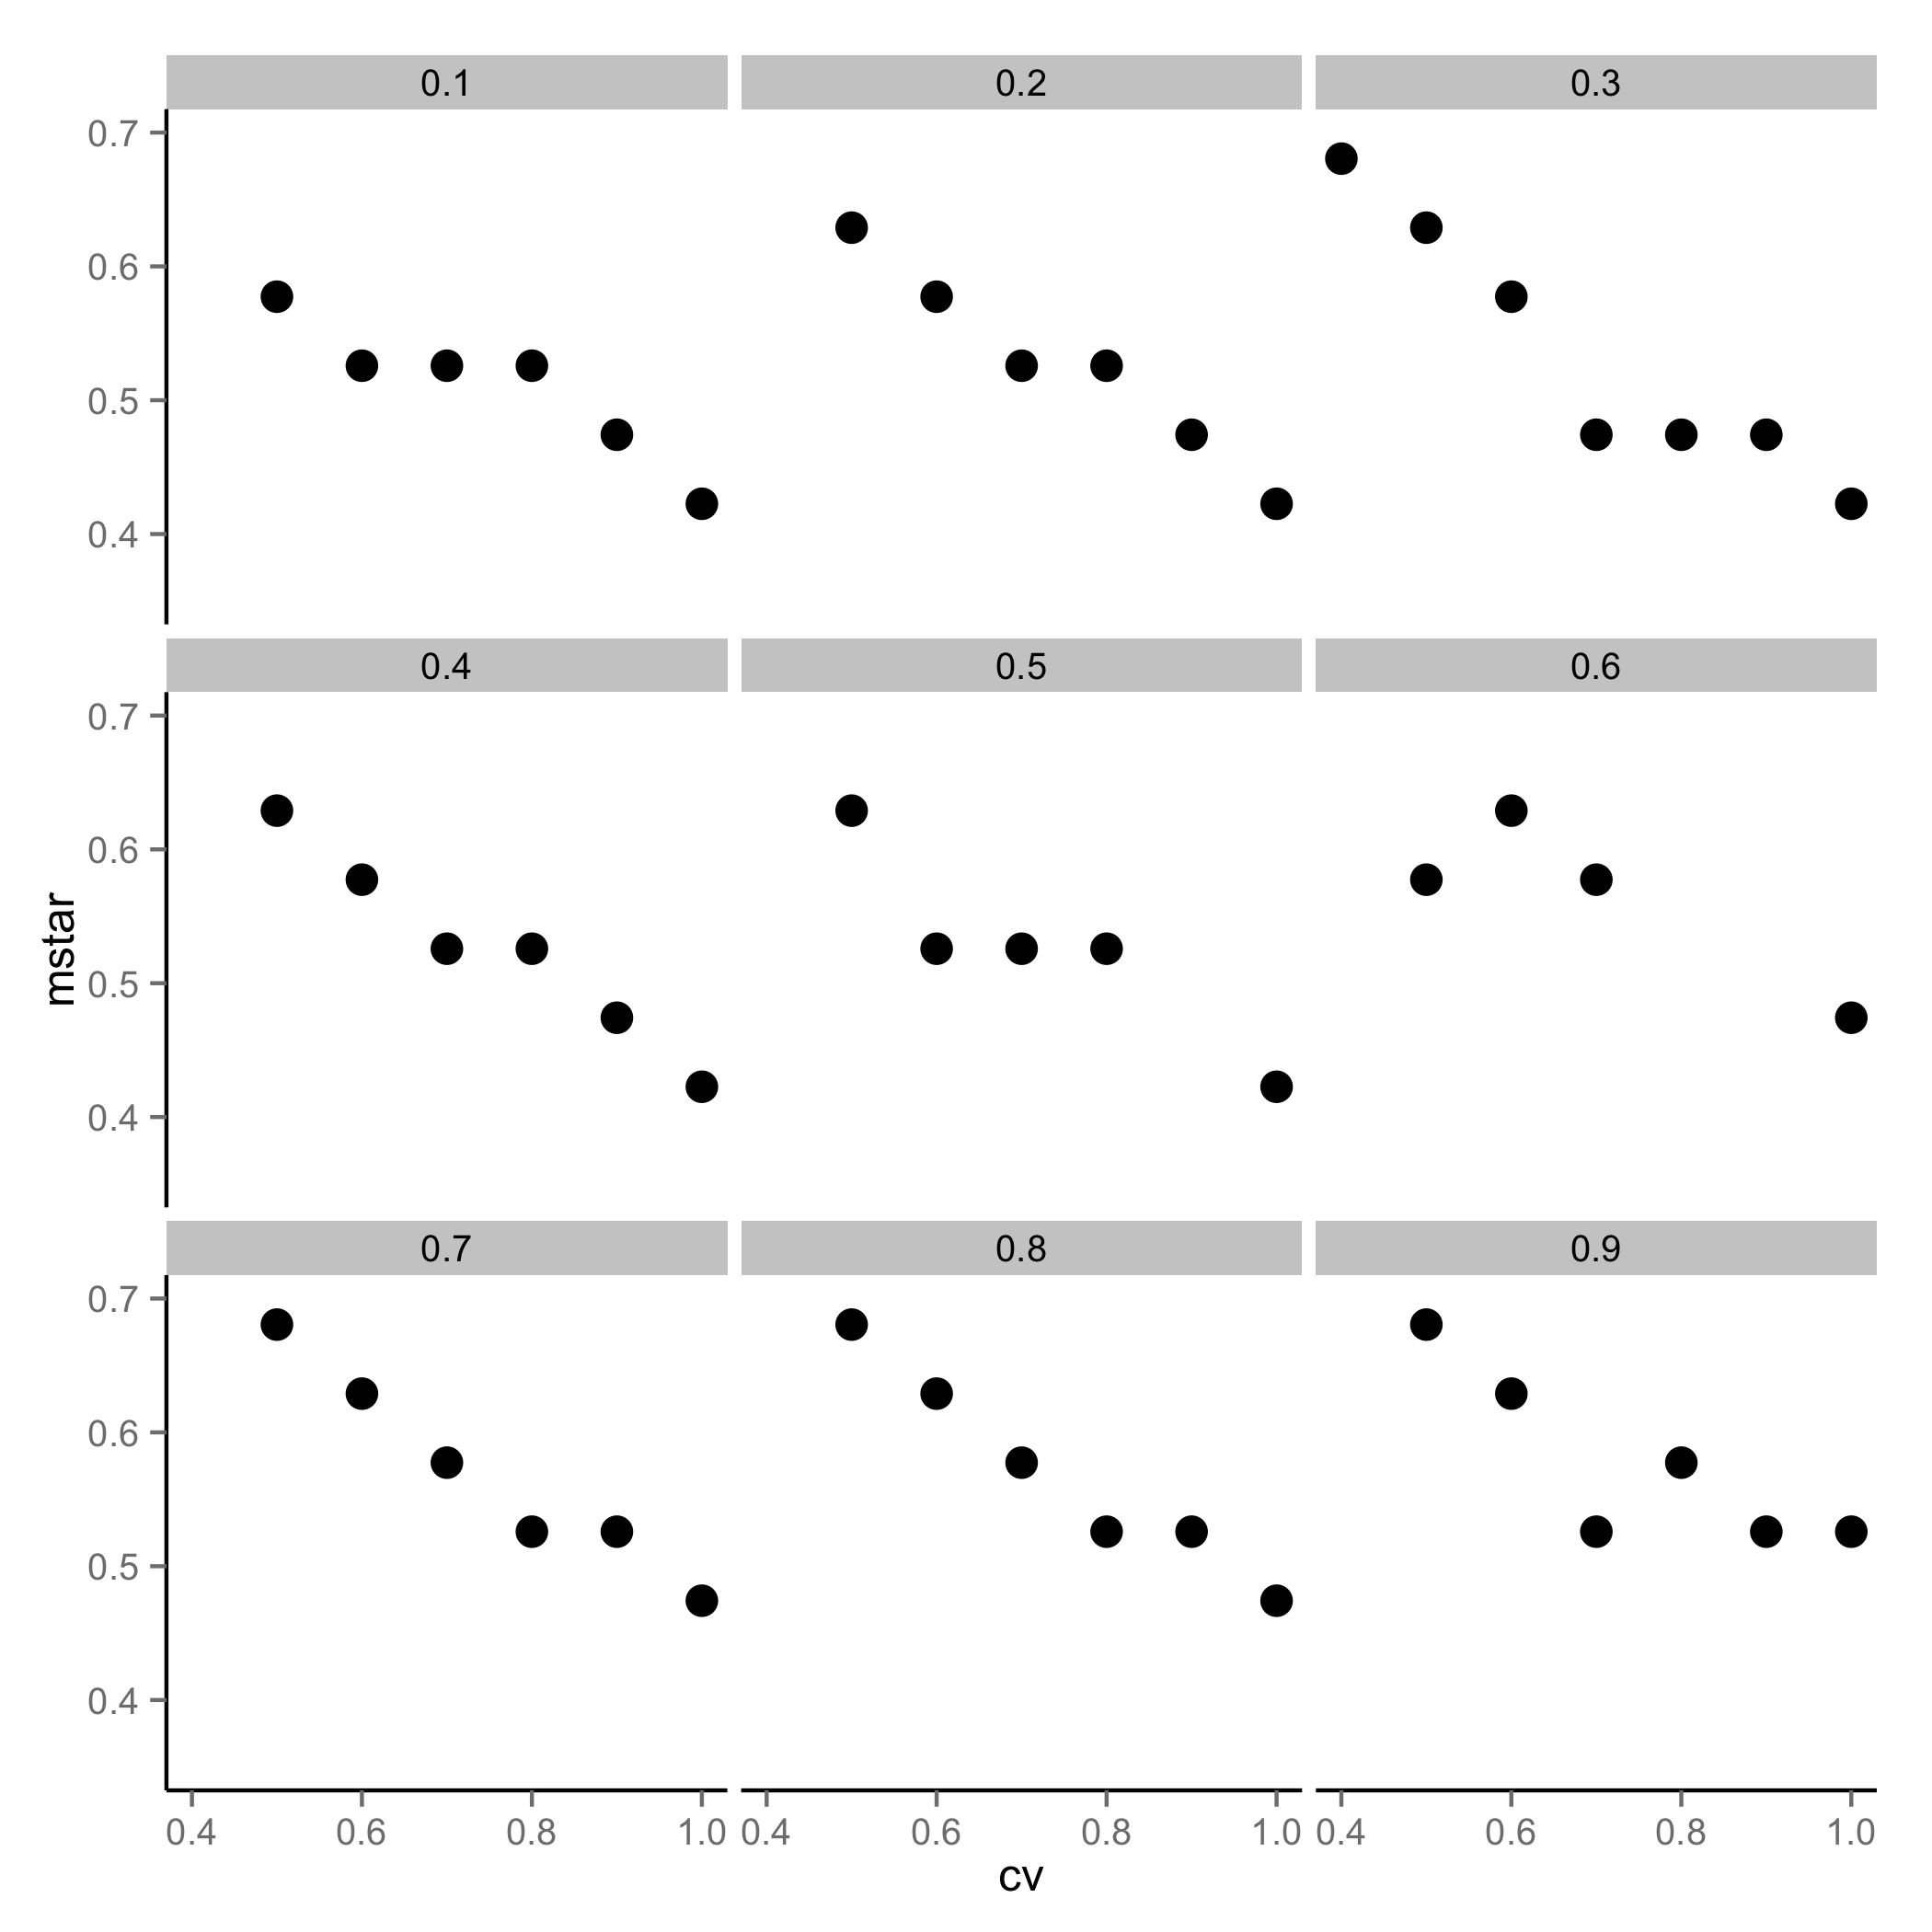
\includegraphics[width=15cm,height=15cm]{td1_nsmooth.png} 

Notice that optimal growth rate does not vary smoothly with cv. Each panel above indicates a different level of correlation.\\

Trade-off 2 (adult survival vs. fecundity): Unless I set this up incorrectly (which I have checked several times), imposing a linear trade off between adult survival and fecundity always results in a boundary condition without any optimum. Table 1 is the trade of foutcome of one such run for a matrix case. \\


% latex table generated in R 2.15.1 by xtable 1.7-0 package
% Wed Sep 12 07:36:49 2012
\begin{table}[ht]
\begin{center}
\begin{tabular}{rrrrrl}
  \hline
 & sA & Fec & lambda & cv & type \\ 
  \hline
1 & 0.01 & 59.40 & 5.84 & 1.00 & simple \\ 
  2 & 0.06 & 56.31 & 5.72 & 1.00 & simple \\ 
  3 & 0.11 & 53.21 & 5.59 & 1.00 & simple \\ 
  4 & 0.16 & 50.12 & 5.45 & 1.00 & simple \\ 
  5 & 0.22 & 47.02 & 5.31 & 1.00 & simple \\ 
  6 & 0.27 & 43.93 & 5.16 & 1.00 & simple \\ 
  7 & 0.32 & 40.83 & 5.01 & 1.00 & simple \\ 
  8 & 0.37 & 37.74 & 4.85 & 1.00 & simple \\ 
  9 & 0.42 & 34.64 & 4.69 & 1.00 & simple \\ 
  10 & 0.47 & 31.55 & 4.51 & 1.00 & simple \\ 
  11 & 0.53 & 28.45 & 4.33 & 1.00 & simple \\ 
  12 & 0.58 & 25.36 & 4.13 & 1.00 & simple \\ 
  13 & 0.63 & 22.26 & 3.92 & 1.00 & simple \\ 
  14 & 0.68 & 19.17 & 3.70 & 1.00 & simple \\ 
  15 & 0.73 & 16.07 & 3.45 & 1.00 & simple \\ 
  16 & 0.78 & 12.98 & 3.18 & 1.00 & simple \\ 
  17 & 0.84 & 9.88 & 2.87 & 1.00 & simple \\ 
  18 & 0.89 & 6.79 & 2.50 & 1.00 & simple \\ 
  19 & 0.94 & 3.69 & 2.03 & 1.00 & simple \\ 
  20 & 0.99 & 0.60 & 1.28 & 1.00 & simple \\ 
   \hline
\end{tabular}
\caption{When imposing a linear tradeoff between adult survival and fecundity, the optimum is always a boundary condition for any scenario.}
\end{center}
\end{table}



 
Trade-off 3 (juveline growth and fecundity): Although I am able to generate a trade off for most parameter combinations, outside of a simple matrix case, the trade off curves contain a lot simulation noise (figure 2 following the table).

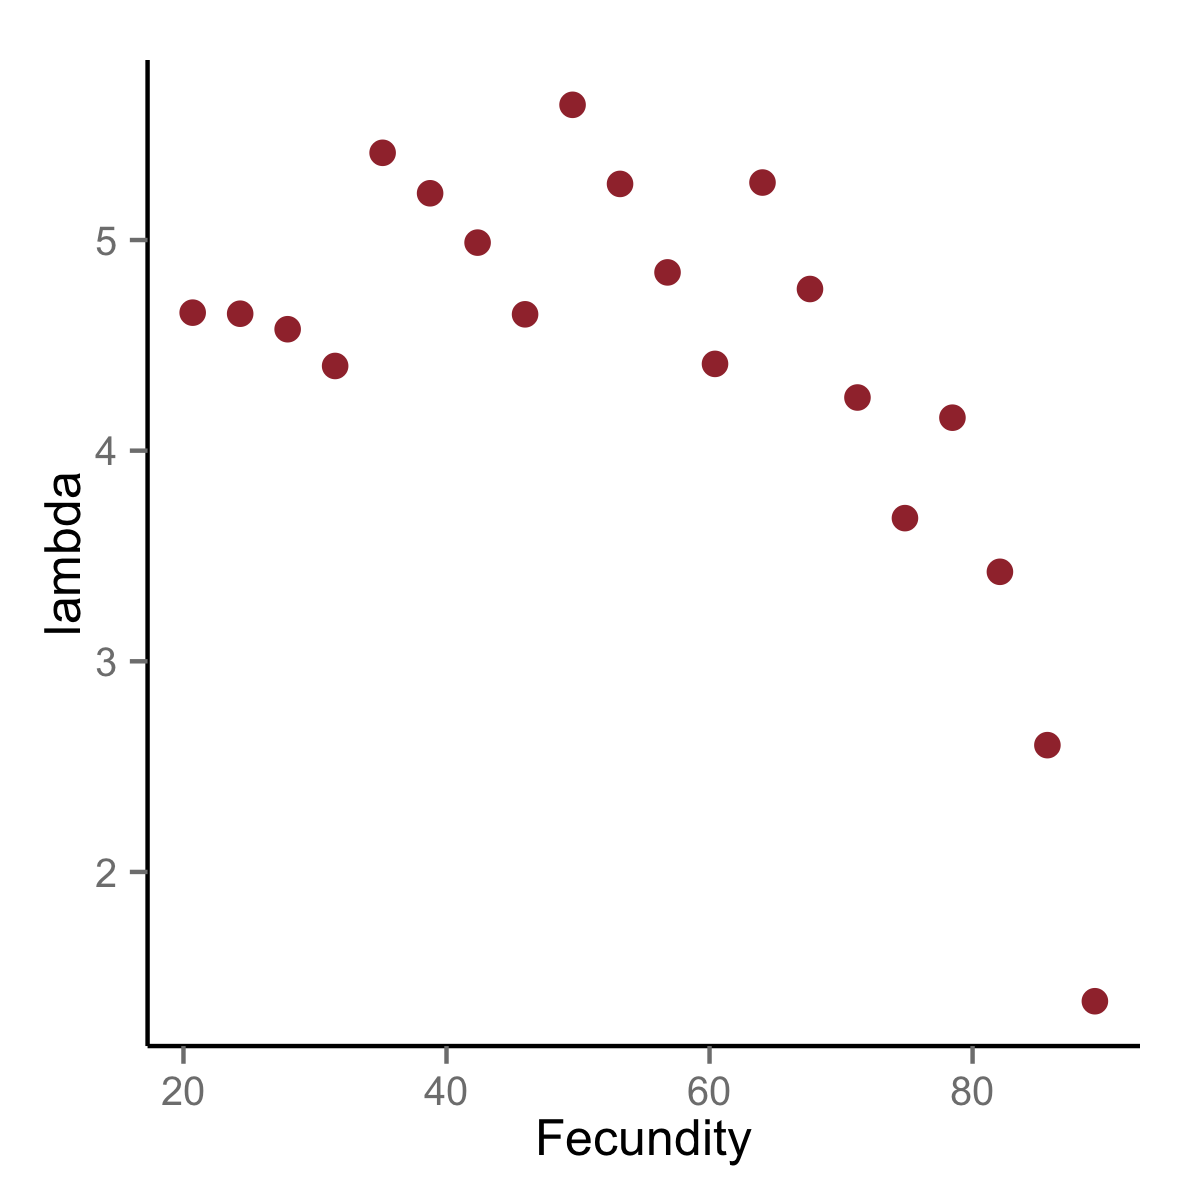
\includegraphics[width=15cm,height=15cm]{t3.png} 

 

\end{document}
